\documentclass{beamer}

\usepackage{ifthen}
\usepackage{pgf}
\usepackage{ulem}
\usepackage{tikz}
\usetikzlibrary{backgrounds}
\usetikzlibrary{calc}
\usetikzlibrary{positioning}
\usetikzlibrary{patterns}
\usetikzlibrary{decorations.pathreplacing}
\usetikzlibrary{arrows,shapes}
\usepackage{tikzpeople}
\usepackage{amssymb}

% Active adversary
\newcommand{\actadv}[4][]{
  \ifthenelse{\equal{#1}{}}{
    \draw[fill=white] #2 rectangle #3 node[pos=.5] {};
    \draw ($#2 + (3,1.5)$) node[devil,mirrored,minimum size=1cm] {};
    \draw[fill=white, fill opacity=0.5] #2 rectangle #3 node[pos=.5] {};
    \draw #2 rectangle #3 node[pos=.5] {\footnotesize #4};
  }{
    \onlyenv<#1>
    \draw[fill=white] #2 rectangle #3 node[pos=.5] {};
    \draw ($#2 + (3,1.5)$) node[devil,mirrored,minimum size=1cm] {};
    \draw[fill=white, fill opacity=0.5] #2 rectangle #3 node[pos=.5] {};
    \draw #2 rectangle #3 node[pos=.5] {\footnotesize #4};
    \endonlyenv
  }
}

% Inactive adversary
\newcommand{\inactadv}[4][]{
  \ifthenelse{\equal{#1}{}}{
    \draw[fill=white] #2 rectangle #3 node[pos=.5] {};
    \draw ($#2 + (3,1.5)$) node[devil,mirrored,minimum size=1cm] {};
    \draw[fill=white, fill opacity=0.4] #2 rectangle #3 node[pos=.5] {};
    \draw[fill=gray, fill opacity=0.5] #2 rectangle #3 node[pos=.5] {};
    \draw #2 rectangle #3 node[pos=.5] {\footnotesize #4};
  }{
    \onlyenv<#1>
    \draw[fill=white] #2 rectangle #3 node[pos=.5] {};
    \draw ($#2 + (3,1.5)$) node[devil,mirrored,minimum size=1cm] {};
    \draw[fill=white, fill opacity=0.4] #2 rectangle #3 node[pos=.5] {};
    \draw[fill=gray, fill opacity=0.5] #2 rectangle #3 node[pos=.5] {};
    \draw #2 rectangle #3 node[pos=.5] {\footnotesize #4};
    \endonlyenv
  }
}

% Active stack frame
\newcommand{\actsf}[4][]{
  \ifthenelse{\equal{#1}{}}{
    \draw[fill=white] #2 rectangle #3 node[pos=.5] {\footnotesize #4};
  }{
   \draw<#1>[fill=white] #2 rectangle #3 node[pos=.5] {#4};
 }
}

% Inactive stack frame
\newcommand{\inactsf}[4][]{
  \ifthenelse{\equal{#1}{}}{
    \draw[fill=white] #2 rectangle #3 node[pos=.5] {};
    \draw[fill=gray, fill opacity=0.5] #2 rectangle #3 node[pos=.5] {};
    \draw #2 rectangle #3 node[pos=.5] {\footnotesize #4};
  }{
    \draw<#1>[fill=white] #2 rectangle #3 node[pos=.5] {};
    \draw<#1>[fill=gray, fill opacity=0.5] #2 rectangle #3 node[pos=.5] {};
    \draw<#1> #2 rectangle #3 node[pos=.5] {\footnotesize #4};
  }
}

\newcommand{\capbrace}[3][sp1]{
  \draw [decorate,decoration={brace,amplitude=10pt,mirror,raise=4pt},yshift=0pt]
  #2 -- #3 node[draw=black] (#1) [black,midway,xshift=0.8cm] {};

}

\newcommand{\stdstackstart}{
  \scope
    \clip (-.1,-.1) rectangle (6.1,15.1);
    \fill[fill=white] (0,0) rectangle (6,15);
    \draw (0,0) -- (0,15);
    \draw (6,0) -- (6,15);
    \draw[fill=gray!50] (0,-.5) rectangle (6,2.5) node[pos=.5,color=black] {\footnotesize higher stack frames...};
  \endscope
  \draw[->] (-2,0) -- node[midway,sloped,above] {stack grows upward} (-2,15);
}


% stolen from https://tex.stackexchange.com/questions/14225/is-there-the-easiest-way-to-toggle-show-hide-navigational-grids-in-tikz/14230
\makeatletter
\newif\if@showgrid@grid
\newif\if@showgrid@left
\newif\if@showgrid@right
\newif\if@showgrid@below
\newif\if@showgrid@above
\tikzset{%
    every show grid/.style={},
    show grid/.style={execute at end picture={\@showgrid{grid=true,#1}}},%
    show grid/.default={true},
    show grid/.cd,
    labels/.style={font={\sffamily\small},help lines},
    xlabels/.style={},
    ylabels/.style={},
    keep bb/.code={\useasboundingbox (current bounding box.south west) rectangle (current bounding box.north west);},
    true/.style={left,below},
    false/.style={left=false,right=false,above=false,below=false,grid=false},
    none/.style={left=false,right=false,above=false,below=false},
    all/.style={left=true,right=true,above=true,below=true},
    grid/.is if=@showgrid@grid,
    left/.is if=@showgrid@left,
    right/.is if=@showgrid@right,
    below/.is if=@showgrid@below,
    above/.is if=@showgrid@above,
    false,
}

\def\@showgrid#1{%
    \begin{scope}[every show grid,show grid/.cd,#1]
    \if@showgrid@grid
    \begin{pgfonlayer}{background}
    \draw [help lines]
        (current bounding box.south west) grid
        (current bounding box.north east);
%
    \pgfpointxy{1}{1}%
    \edef\xs{\the\pgf@x}%
    \edef\ys{\the\pgf@y}%
    \pgfpointanchor{current bounding box}{south west}
    \edef\xa{\the\pgf@x}%
    \edef\ya{\the\pgf@y}%
    \pgfpointanchor{current bounding box}{north east}
    \edef\xb{\the\pgf@x}%
    \edef\yb{\the\pgf@y}%
    \pgfmathtruncatemacro\xbeg{ceil(\xa/\xs)}
    \pgfmathtruncatemacro\xend{floor(\xb/\xs)}
    \if@showgrid@below
    \foreach \X in {\xbeg,...,\xend} {
        \node [below,show grid/labels,show grid/xlabels] at (\X,\ya) {\X};
    }
    \fi
    \if@showgrid@above
    \foreach \X in {\xbeg,...,\xend} {
        \node [above,show grid/labels,show grid/xlabels] at (\X,\yb) {\X};
    }
    \fi
    \pgfmathtruncatemacro\ybeg{ceil(\ya/\ys)}
    \pgfmathtruncatemacro\yend{floor(\yb/\ys)}
    \if@showgrid@left
    \foreach \Y in {\ybeg,...,\yend} {
        \node [left,show grid/labels,show grid/ylabels] at (\xa,\Y) {\Y};
    }
    \fi
    \if@showgrid@right
    \foreach \Y in {\ybeg,...,\yend} {
        \node [right,show grid/labels,show grid/ylabels] at (\xb,\Y) {\Y};
    }
    \fi
    \end{pgfonlayer}
    \fi
    \end{scope}
}
\makeatother

\begin{document}
\begin{frame}
  \frametitle{Traditional stack pointers}
  \begin{tikzpicture}[scale=.5, every node={scale=.5}]
    % recurrent parts
    \begin{scope}
      \clip (-.1,-.1) rectangle (6.1,15.1);
      \fill[gray!20,draw=none,opacity=.8] (0,0) rectangle (6,15);
      \draw[draw=gray!80] (0,0) -- (0,15);
      \draw[draw=gray!80] (6,0) -- (6,15);
      \draw[fill=white] (0,-.5) rectangle (6,2.5) node[pos=.5] {\footnotesize higher stack frames...};
    \end{scope}
    \draw[->] (-1,0) -- node[midway,sloped,above] {stack grows upward} (-1,15);

    % traditional:
    \draw<+>[fill=white] (0,2.5) rectangle (6,5.5) node[pos=.5] {\footnotesize caller stack frame};
    \draw<.> (8,7) node[draw=black] (sp0) {};
    \draw<.> node[right=0cm of sp0] (sp0l) { stack pointer };
    \draw<.> (sp0) edge[->,out=235,in=0] (6,5.25);

    % traditional call:
    \draw<+>[fill=white] (0,2.5) rectangle (6,5.5) node[pos=.5] {\footnotesize caller stack frame};
    \draw<.>[fill=white] (0,5.5) rectangle (6,8.5) node[pos=.5] {\footnotesize callee stack frame};
    \draw<.> (8,7) node[draw=black] (sp0) {};
    \draw<.> node[right=0cm of sp0] (sp0l) { stack pointer };
    \draw<.> (sp0) edge[->,out=235,in=0] (6,8.25);

    % traditional return:
    \draw<+>[fill=white] (0,2.5) rectangle (6,5.5) node[pos=.5] {\footnotesize caller stack frame};
    \draw<.> (8,7) node[draw=black] (sp0) {};
    \draw<.> node[right=0cm of sp0] (sp0l) { stack pointer };
    \draw<.> (sp0) edge[->,out=235,in=0] (6,5.25);

    % traditional call, attack:
    \draw<+->[fill=white] (0,2.5) rectangle (6,5.5) node[pos=.5] {\footnotesize caller stack frame};
    \draw<.->[fill=white] (0,5.5) rectangle (6,8.5) node[pos=.5] {\footnotesize callee stack frame};
    \draw<.-> (8,7) node[draw=black] (sp0) {};
    \draw<.-> node[right=0cm of sp0] (sp0l) { stack pointer };

    % read other stack frames
    \draw<.> (sp0) edge[->,out=235,in=0] (6,8.25);
    \actadv[.]{(0,5.5)}{(6,8.5)}{callee stack frame}
    \draw<.> (sp0) edge[->,color=red,very thick,out=235,in=0] node[sloped, below] {read/write} (6,4);

    % break well-bracketedness
    \draw<+>[fill=red,opacity=.7] (-.5,2.5) rectangle (6.5,8.5);
    \draw<.-> (8,7) node[draw=black] (sp0) {};
    \draw<.>[red] (sp0) edge[->,out=235,in=0] (6,1.75);
    \draw<.> node[color=red,align=left,below=of sp0l] {return but\\
      skip caller frame};
  \end{tikzpicture}

\end{frame}

\begin{frame}
  \frametitle{Stack and return capabilities}
  \begin{tikzpicture}[scale=.5, every node={scale=.5}]
    % recurrent parts
    \stdstackstart

    % first step: capabilities
    \begin{onlyenv}<+-+(4)>
      \draw[fill=white] (0,2.5) rectangle (6,5.5) node[pos=.5] {\footnotesize current stack frame};
    \end{onlyenv}
    \begin{onlyenv}<.-.(3)>
      \draw [decorate,decoration={brace,amplitude=10pt,mirror,raise=4pt},yshift=0pt]
      (6.5,2.5) -- (6.5,16) node[draw=black] (sp1) [black,midway,xshift=0.8cm] {};
      \draw node[right=0cm of sp1] { stack pointer };
    \end{onlyenv}
    \begin{onlyenv}<.-.(1)>
      \draw [decorate,decoration={brace,amplitude=10pt,mirror,raise=4pt},yshift=0pt]
      (6,0) -- (6,16) node (oldframe1) [black,midway,xshift=0.5cm] {};
      \draw node[fill=gray!50,right=0cm of oldframe1] (rp1l) {return pointer data};
    \end{onlyenv}

    %prepare call: store old return pointer
    \draw<+-+(3)>[fill=gray!50] (0,6) rectangle node {\scriptsize old return pointer code} (6,6.5);
    \begin{onlyenv}<+-+(2)>
      \draw[fill=gray!50] (0,5.5) rectangle node {\scriptsize old return pointer data} (6,6);
      \draw [decorate,decoration={brace,amplitude=10pt,raise=4pt},yshift=0pt]
      (0,0) -- (0,16) node (oldframe1) [black,midway,xshift=-0.5cm] {};
      \draw (0,5.75) edge[->,out=180,in=225] (oldframe1); 
    \end{onlyenv}
    \begin{onlyenv}<+->
      \draw [decorate,decoration={brace,amplitude=10pt,mirror,raise=4pt,aspect=.4},yshift=0pt]
      (6,2.5) -- (6,16) node (callerframe1) [draw=black,pos=.4,xshift=0.8cm] {};
      \draw node[fill=gray!50,right=0cm of callerframe1] (rp1l) {new return pointer data};
    \end{onlyenv}
    \begin{onlyenv}<+->
      \draw [decorate,decoration={brace,amplitude=10pt,mirror,raise=4pt},yshift=0pt]
      (6.5,6.5) -- (6.5,16) node[draw=black] (sp1) [black,midway,xshift=0.8cm] {};
      \draw node[right=0cm of sp1] { new stack pointer };
    \end{onlyenv}
    
    % call using capabilities
    \begin{onlyenv}<+->
      \draw[fill=gray!50] (0,2.5) rectangle (6,6.5) node[pos=.5] {\footnotesize caller stack frame};
      \draw[fill=white] (0,6.5) rectangle (6,9.5) node[pos=.5] {\footnotesize callee stack frame};
    \end{onlyenv}
  \end{tikzpicture}
\end{frame} 

\begin{frame}
  \frametitle{Stack and return capabilities: Attack 1}
  \begin{tikzpicture}[scale=.5, every node={scale=.5}]
    % recurrent parts
    \stdstackstart

    % attacker...
    \begin{onlyenv}<+-+(2)>
      \draw[fill=gray!50] (0,2.5) rectangle (6,6.5) node[pos=.5] {\footnotesize caller stack frame};
      \actadv{(0,6.5)}{(6,9.5)}{callee stack frame}
      \draw [decorate,decoration={brace,amplitude=10pt,mirror,raise=4pt},yshift=0pt]
      (6.5,6.5) -- (6.5,16) node[draw=black] (sp1) [black,midway,xshift=0.8cm] {};
      \draw node[right=0cm of sp1] { stack pointer };
    \end{onlyenv}

    % stores stack pointer in heap
    \begin{onlyenv}<+->
      \begin{scope}
        \fill[gray!20] (14,6) rectangle (18,13);
        \draw (14,6) -- (14,13);
        \draw (18,6) -- (18,13);
      \end{scope}
      \draw (16,14) node {heap memory};
      \draw[fill=gray!50] (14,8) rectangle node[color=red] {\scriptsize copy of old sp} (18,8.5);
    \end{onlyenv}
    \draw<.> (14,8.25) edge[->,red,thick,bend left] (sp1);
    \begin{onlyenv}<+->
      \draw [decorate,decoration={brace,amplitude=10pt,mirror,raise=4pt},yshift=0pt]
      (11.5,6.5) -- (11.5,16) node[draw=black] (spold) [black,midway,xshift=0.8cm] {};
      \draw (14,8.25) edge[->,red,thick,bend left] (spold);
    \end{onlyenv}

    % attacker returns
    \begin{onlyenv}<+>
      \draw [decorate,decoration={brace,amplitude=10pt,mirror,raise=4pt},yshift=0pt]
      (6.5,2.5) -- (6.5,16) node[draw=black] (sp1) [black,midway,xshift=0.8cm] {};
      \draw node[right=0cm of sp1] { stack pointer };
      \draw[fill=white] (0,2.5) rectangle (6,6.5) node[pos=.5] {\footnotesize current stack frame};
    \end{onlyenv}

    % attacker gets called again + uses old stack pointer.
    \begin{onlyenv}<+>
      \draw[fill=gray!50] (0,2.5) rectangle (6,10.5) node[pos=.5] {\footnotesize caller stack frame};
      \actadv{(0,10.5)}{(6,13.5)}{callee stack frame}
      \draw (14,8.25) edge[->,color=red,very thick,out=235,in=0] node[sloped, below] {read/write} (6,8);
      \draw [decorate,decoration={brace,amplitude=10pt,mirror,raise=4pt},yshift=0pt]
        (6.5,10.5) -- (6.5,16) node[draw=black] (sp1) [black,midway,xshift=0.8cm] {};
      \draw node[right=0cm of sp1] { stack pointer };
      % \draw [decorate,decoration={brace,amplitude=10pt,mirror,raise=4pt},yshift=0pt]
      % (6,2.5) -- (6,16) node (callerframe1) [draw=black,midway,xshift=0.8cm] {};
      % \draw node[fill=gray!50,right=0cm of callerframe1] (rp1l) {return pointer data};
    \end{onlyenv}
  \end{tikzpicture}
\end{frame}

\begin{frame}
  \frametitle{Stack and return capabilities: Attack 2}
  \begin{tikzpicture}[scale=.5, every node={scale=.5}]
    % recurrent parts
    \stdstackstart

    % first step: capabilities
    \begin{onlyenv}<+>
      \draw[fill=white] (0,2.5) rectangle (6,4) node[pos=.5] {\footnotesize current stack frame};
      \draw [decorate,decoration={brace,amplitude=10pt,mirror,raise=4pt},yshift=0pt]
        (6.5,2.5) -- (6.5,16) node[draw=black] (sp1) [black,midway,xshift=0.8cm] {};
      \draw node[right=0cm of sp1] { stack pointer };
      % \draw [decorate,decoration={brace,amplitude=10pt,mirror,raise=4pt},yshift=0pt]
      % (6,0) -- (6,16) node (oldframe1) [black,midway,xshift=0.5cm] {};
      % \draw node[fill=gray!50,right=0cm of oldframe1] (rp1l) {return pointer data};
    \end{onlyenv}

    % attacker stores copy of stack pointer high in the stack
    \draw<+->[fill=gray!50] (0,2.5) rectangle (6,4) node[pos=.5] {\footnotesize caller stack frame};
    \begin{onlyenv}<.-.(2)>
      \actadv{(0,4)}{(6,7)}{callee stack frame}
      \draw [decorate,decoration={brace,amplitude=10pt,mirror,raise=4pt},yshift=0pt]
        (6.5,4) -- (6.5,16) node[draw=black] (sp1) [black,midway,xshift=0.8cm] {};
      \draw node[right=0cm of sp1] { stack pointer };
    \end{onlyenv}
    \draw<+->[fill=white] (0,13) rectangle (6,13.5) node[pos=.5,color=red] {\footnotesize copy of sp};
    \draw<.> (6,13.25) edge[red,thick,->,in=45] (sp1);
    \begin{onlyenv}<+->
      \draw [decorate,decoration={brace,amplitude=10pt,mirror,raise=4pt},yshift=0pt]
        (13.5,4) -- (13.5,16) node[draw=black] (spold) [black,midway,xshift=0.8cm] {};
      \draw (6,13.25) edge[red,thick,->,in=45] (spold);
    \end{onlyenv}

    % attacker calls trusted code again
%    \draw<+->[fill=gray!50] (0,4) rectangle (6,7) node[pos=.5] {\footnotesize callee stack frame};
    \begin{onlyenv}<+->
      \inactadv{(0,4)}{(6,7)}{callee stack frame}
    \end{onlyenv}
    \begin{onlyenv}<.>
      \draw[fill=white] (0,7) rectangle (6,9) node[pos=.5] {\footnotesize callee (2) stack frame};
      \draw [decorate,decoration={brace,amplitude=10pt,mirror,raise=4pt},yshift=0pt]
        (6.5,7) -- (6.5,16) node[draw=black] (sp1) [black,midway,xshift=0.8cm] {};
      \draw node[right=0cm of sp1] { stack pointer };
    \end{onlyenv}

    % attacker uses old stack pointer
    \draw<+->[fill=gray!50] (0,7) rectangle (6,9) node[pos=.5] {\footnotesize callee (2) stack frame};
    \begin{onlyenv}<.-.(1)>
      \actadv{(0,9)}{(6,12)}{callee (3) stack frame}
      \draw [decorate,decoration={brace,amplitude=10pt,mirror,raise=4pt},yshift=0pt]
      (6.5,9) -- (6.5,16) node[draw=black] (sp1) [black,midway,xshift=0.8cm] {};
      \draw node[right=0cm of sp1] { stack pointer };
    \end{onlyenv}
    \draw<+> (spold) edge[->,color=red,very thick,out=235,in=0] node[sloped, below] {read/write} (6,8);
  \end{tikzpicture}
\end{frame}

\begin{frame}
  \frametitle{Stack Capabilities Problems}
  \begin{itemize}
  \item Stack capabilities are not a panacea
  \item Stack pointers must not leave stack frame (through memory or stack)
  \item Similar problems for return pointers (omitted)
  \item Solution: local capabilities?
    \begin{itemize}
    \item Make stack and return capabilities local
    \item Cannot leave registers (except on stack) (\sout{Attack 1})
    \item Stack clearing on boundary crossings (\sout{Attack 2})
    \end{itemize}
  \end{itemize}
\end{frame}

\begin{frame}
  \frametitle{Local Stack Capabilities prevent Attack 1}
  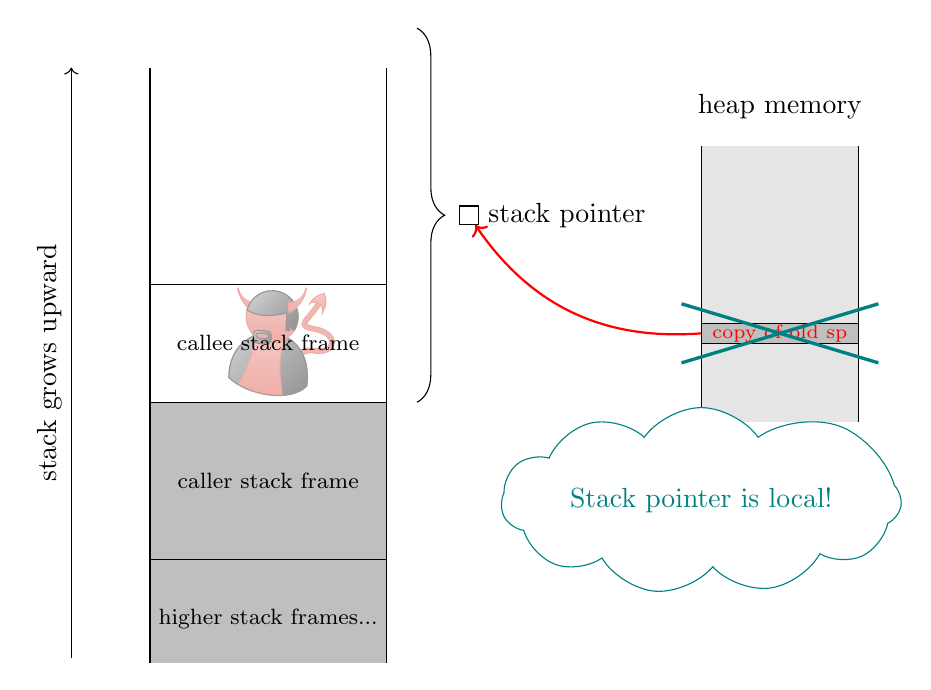
\begin{tikzpicture}[scale=.5, every node={scale=.5}]
    % recurrent parts
    \stdstackstart
    
    % attacker...
    \draw[fill=gray!50] (0,2.5) rectangle (6,6.5) node[pos=.5] {\footnotesize caller stack frame};
    \actadv{(0,6.5)}{(6,9.5)}{callee stack frame}
    \draw [decorate,decoration={brace,amplitude=10pt,mirror,raise=4pt},yshift=0pt]
      (6.5,6.5) -- (6.5,16) node[draw=black] (sp1) [black,midway,xshift=0.8cm] {};
    \draw node[right=0cm of sp1] { stack pointer };

    % stores stack pointer in heap
    \begin{scope}
      \fill[gray!20] (14,6) rectangle (18,13);
      \draw (14,6) -- (14,13);
      \draw (18,6) -- (18,13);
    \end{scope}
    \draw (16,14) node {heap memory};
    \draw[fill=gray!50] (14,8) rectangle node[color=red] {\scriptsize copy of old sp} (18,8.5);
    \draw (14,8.25) edge[->,red,thick,bend left] (sp1);
    \draw[teal,very thick] (13.5,7.5) -- (18.5,9);
    \draw[teal,very thick] (18.5,7.5) -- (13.5,9);
    \draw node[teal,cloud,cloud puffs=10.8,cloud puff arc=110, aspect=3, draw, fill=white] () at (14,4) {Stack pointer is local!};  
\end{tikzpicture}
\end{frame}

\begin{frame}
  \frametitle{Local caps: Stack clearing prevents Attack 2}
  \begin{tikzpicture}[scale=.5, every node={scale=.5}]
    % recurrent parts
    \stdstackstart

    % attacker stores copy of stack pointer high in the stack
    \draw[fill=gray!50] (0,2.5) rectangle (6,4) node[pos=.5] {\footnotesize caller stack frame};
    \begin{onlyenv}<+>
      \actadv{(0,4)}{(6,7)}{callee stack frame}
    \end{onlyenv}
    \draw<.-.(2)>[fill=white] (0,13) rectangle (6,13.5) node[pos=.5,color=red] {\footnotesize copy of sp};
    \draw<.-.(2)> [decorate,decoration={brace,amplitude=10pt,mirror,raise=4pt},yshift=0pt]
    (13.5,4) -- (13.5,16) node[draw=black] (spold) [black,midway,xshift=0.8cm] {};
    \draw<.-.(2)> (6,13.25) edge[red,thick,->,in=45] (spold);

    % attacker calls trusted code again
    \begin{onlyenv}<+->
      \inactadv{(0,4)}{(6,7)}{callee stack frame}
    \end{onlyenv}
    \begin{onlyenv}<.-.(1)>
      \draw[fill=white] (0,7) rectangle (6,9) node[pos=.5] {\footnotesize callee (2) stack frame};
      \draw [decorate,decoration={brace,amplitude=10pt,mirror,raise=4pt},yshift=0pt]
        (6.5,7) -- (6.5,16) node[draw=black] (sp1) [black,midway,xshift=0.8cm] {};
      \draw node[right=0cm of sp1] { stack pointer };
    \end{onlyenv}

    % trusted code clears the stack
    \begin{onlyenv}<+->
      \foreach \x in {9,9.5,...,14}
      {
        \draw[fill=white] (0,\x) rectangle (6,\x+.5) node[pos=.5,color=teal] {\footnotesize 0};
      };
    \end{onlyenv}
    \draw<.>[very thick,color=teal] (10,13.5) -- (13,14.5)
    (13,13.5) -- (10,14.5);
    
    % attacker uses old stack pointer
    \draw<+->[fill=gray!50] (0,7) rectangle (6,9) node[pos=.5] {\footnotesize callee (2) stack frame};
    \begin{onlyenv}<.>
      \actadv{(0,9)}{(6,12)}{callee (3) stack frame}
      \draw [decorate,decoration={brace,amplitude=10pt,mirror,raise=4pt},yshift=0pt]
      (6.5,9) -- (6.5,16) node[draw=black] (sp1) [black,midway,xshift=0.8cm] {};
      \draw node[right=0cm of sp1] { stack pointer };
    \end{onlyenv}

    % attacker returns
    \draw<+>[fill=white] (0,9) rectangle (6,12) node[pos=.5] {?};
    \begin{onlyenv}<.>
      \draw[fill=white] (0,7) rectangle (6,9) node[pos=.5] {\footnotesize callee (2) stack frame};
      \draw [decorate,decoration={brace,amplitude=10pt,mirror,raise=4pt},yshift=0pt]
        (6.5,7) -- (6.5,16) node[draw=black] (sp1) [black,midway,xshift=0.8cm] {};
      \draw node[right=0cm of sp1] { stack pointer };
    \end{onlyenv}

    % trusted code clears stack again
    \begin{onlyenv}<+->
      \foreach \x in {7,7.5,...,14}
      {
        \draw[fill=white] (0,\x) rectangle (6,\x+.5) node[pos=.5,color=teal] {\footnotesize 0};
      };
    \end{onlyenv}
    % then, the trusted code can return
    \begin{onlyenv}<+>
      \actadv{(0,4)}{(6,7)}{callee stack frame}
    \end{onlyenv}
    
  \end{tikzpicture}
\end{frame}

\begin{frame}
    \frametitle{Linear caps: stack pointers}
  \begin{tikzpicture}[scale=.5, every node={scale=.5}]
    % recurrent parts
    \stdstackstart

    % Caller 
    \actsf{(0,2.5)}{(6,5)}{caller stack frame} 
    \begin{onlyenv}<+>
      \capbrace{(6.5,2.5)}{(6.5,16)}
      \draw node[right=0cm of sp1] { stack pointer };
    \end{onlyenv}


    % Split the stack pointer
    \begin{onlyenv}<+>
      \capbrace[sp2]{(6.5,2.5)}{(6.5,5)}
      \capbrace[usp]{(6.5,5)}{(6.5,16)}
      \draw node[right=0cm of usp] { stack pointer };
      \draw node[right=0cm of sp2] { private stack pointer };
    \end{onlyenv}


    % Callee called
    \begin{onlyenv}<+>
      \capbrace[sp2]{(6.5,2.5)}{(6.5,5)}
      \capbrace[usp]{(6.5,5)}{(6.5,16)}
      \draw node[right=0cm of usp] { stack pointer };
      \draw node[fill=gray!50, right=0cm of sp2] { return data pointer };
      \inactsf{(0,2.5)}{(6,5)}{caller stack frame} 
      \actsf{(0,5)}{(6,6.5)}{callee stack frame}
    \end{onlyenv}

    % Return from callee
    \begin{onlyenv}<+>
      \capbrace[sp2]{(6.5,2.5)}{(6.5,5)}
      \capbrace[usp]{(6.5,5)}{(6.5,16)}
      \draw node[right=0cm of usp] { stack pointer };
      \draw node[right=0cm of sp2] { private stack pointer };
    \end{onlyenv}

    % Caller splices the stack frames
    \begin{onlyenv}<+>
      \capbrace{(6.5,2.5)}{(6.5,16)}
      \draw node[right=0cm of sp1] { stack pointer };
    \end{onlyenv}

  \end{tikzpicture}
\end{frame}

\begin{frame}
    \frametitle{Linear caps prevent attack 1}
  \begin{tikzpicture}[scale=.5, every node={scale=.5}]
    % recurrent parts
    \stdstackstart

    % Caller 
    \actsf{(0,2.5)}{(6,5)}{caller stack frame} 
    \begin{onlyenv}<+>
      \capbrace{(6.5,2.5)}{(6.5,16)}
      \draw node[right=0cm of sp1] { stack pointer };
    \end{onlyenv}


    % Split the stack pointer
    \begin{onlyenv}<+>
      \capbrace[sp2]{(6.5,2.5)}{(6.5,5)}
      \draw [decorate,decoration={brace,aspect=0.2,amplitude=10pt,mirror,raise=4pt},yshift=0pt]
      (6.5,5) -- (6.5,16) node[draw=black] (usp) [black,pos=0.2,xshift=0.8cm] {};
      \draw node[right=0cm of usp] { stack pointer };
      \draw node[right=0cm of sp2] { private stack pointer };
    \end{onlyenv}


    % Callee called
    \begin{onlyenv}<+>
      \capbrace[sp2]{(6.5,2.5)}{(6.5,5)}
      \draw [decorate,decoration={brace,aspect=0.2,amplitude=10pt,mirror,raise=4pt},yshift=0pt]
      (6.5,5) -- (6.5,16) node[draw=black] (usp) [black,pos=0.2,xshift=0.8cm] {};
      \draw node[right=0cm of usp] { stack pointer };
      \draw node[fill=gray!50, right=0cm of sp2] { return data pointer };
      \inactsf{(0,2.5)}{(6,5)}{caller stack frame} 
      \actadv{(0,5)}{(6,8)}{callee stack frame}
    \end{onlyenv}


    \begin{onlyenv}<.->
      \begin{scope}
        \fill[gray!20] (14,9) rectangle (18,14);
        \draw (14,9) -- (14,14);
        \draw (18,9) -- (18,14);
      \end{scope}
    \end{onlyenv}
    \draw<.>[fill=white] (14,10) rectangle node[color=red] {} (18,10.5);

    % Callee stores stack pointer
    \begin{onlyenv}<+->
      \draw [decorate,decoration={brace,aspect=0.2,amplitude=10pt,mirror,raise=4pt},yshift=0pt]
      (8,5) -- (8,16) node[draw=black] (usp) [black,pos=0.2,xshift=0.8cm] {};
      \draw (14,10.25) edge[->,red,thick,bend right] (usp);
      \draw (16,15) node {heap memory};
    \end{onlyenv}
    \begin{onlyenv}<.>
      \draw[fill=white] (14,10) rectangle node[color=red] {\scriptsize old sp} (18,10.5);
      \draw node[right=0cm of usp] { stack pointer };
      \inactsf{(0,2.5)}{(6,5)}{caller stack frame} 
      \actadv{(0,5)}{(6,8)}{callee stack frame}
      \capbrace[sp2]{(6.5,2.5)}{(6.5,5)}
      \draw node[fill=gray!50, right=0cm of sp2] { return data pointer };
    \end{onlyenv}

    % Return from callee
    \begin{onlyenv}<+->
      \draw[fill=gray!50] (14,10) rectangle node[color=red] {\scriptsize old sp} (18,10.5);
      \actsf{(0,2.5)}{(6,5)}{caller stack frame} 
      \capbrace[sp2]{(6.5,2.5)}{(6.5,5)}
      \draw node[right=0cm of sp2] { private stack pointer };
      \draw node[right=0cm of usp] { stack pointer };
    \end{onlyenv}

    \draw<+>[teal,very thick] (6.4,4.4) -- (7.4,5.4);
    \draw<.>[teal,very thick] (7.4,4.4) -- (6.4,5.4);
    \draw<.> node[teal,cloud,cloud puffs=10.8,cloud puff arc=110, aspect=3, draw, fill=white, align=center] () at (14,4) { Splice fails,\\ stack pointer is linear!};  
  \end{tikzpicture}  
\end{frame}

\begin{frame}
  \frametitle{Linear caps prevents attack 2}
  \begin{tikzpicture}[scale=.5, every node={scale=.5}]
    % recurrent parts
    \stdstackstart

    % Caller 
    \actsf{(0,2.5)}{(6,5)}{caller stack frame} 
    \begin{onlyenv}<+>
      \capbrace{(6.5,2.5)}{(6.5,16)}
      \draw node[right=0cm of sp1] { stack pointer };
    \end{onlyenv}


    % Split the stack pointer
    \begin{onlyenv}<+>
      \capbrace[sp2]{(6.5,2.5)}{(6.5,5)}
      \capbrace[usp]{(6.5,5)}{(6.5,16)}
      \draw node[right=0cm of usp] { stack pointer };
      \draw node[right=0cm of sp2] { private stack pointer };
    \end{onlyenv}


    % Callee called
    \begin{onlyenv}<+>
      \capbrace[usp]{(6.5,5)}{(6.5,16)}
      \capbrace[sp2]{(6.5,2.5)}{(6.5,5)}
      \draw node[right=0cm of usp] { stack pointer };
      \draw node[fill=gray!50, right=0cm of sp2] { return data pointer };
      \inactsf{(0,2.5)}{(6,5)}{caller stack frame} 
      \actadv{(0,5)}{(6,8)}{callee stack frame}
    \end{onlyenv}

    \begin{onlyenv}<+-.(2)>
      \capbrace[sp2]{(6.5,2.5)}{(6.5,5)}
      \draw node[fill=gray!50, right=0cm of sp2] { return data pointer };

      \capbrace[usp]{(13.5,5)}{(13.5,16)}
      \draw (6,13.25) edge[red,thick,->,in=45] (usp);
      \draw node[right=0cm of usp] { stack pointer };

      \draw[fill=white] (0,13) rectangle (6,13.5) node[pos=.5,color=red] {\footnotesize sp};
      \inactsf{(0,2.5)}{(6,5)}{caller stack frame} 
      \actadv{(0,5)}{(6,8)}{callee stack frame}
    \end{onlyenv}

    % At this point we have a linear point stored in a part of memory that it governs. In other words, no other capabilities can grant access to this part of memory, to the capabilitiy is essentially lost.
    \draw<+> node[teal,cloud,cloud puffs=10.8,cloud puff arc=110, aspect=3, draw, fill=white, align=center] () at (4,10) { Stack pointer\\essentially lost.}; 

    \begin{onlyenv}<+->
      \capbrace[sp2]{(6.5,2.5)}{(6.5,5)}
      \draw node[right=0cm of sp2] { return data pointer };

      \capbrace[usp]{(13.5,5)}{(13.5,16)}
      \draw (6,13.25) edge[red,thick,->,in=45] (usp);
      \draw node[right=0cm of usp] { stack pointer };

      \begin{scope}
        \fill[fill=gray!50] (0,2.5) rectangle (6,15) node[pos=.5,color=black] {};
        \draw (0,0) -- (0,15);
        \draw (6,0) -- (6,15);
      \end{scope}
      \draw[fill=gray!50] (0,13) rectangle (6,13.5) node[pos=.5,color=red] {\footnotesize sp};
      \actsf{(0,2.5)}{(6,5)}{caller stack frame} 
  \end{onlyenv}

  \draw<+>[teal,very thick] (6.4,4.4) -- (7.4,5.4);
  \draw<.>[teal,very thick] (7.4,4.4) -- (6.4,5.4);
  \draw<.> node[teal,cloud,cloud puffs=10.8,cloud puff arc=110, aspect=3, draw, fill=white, align=center] () at (14,7) { Splice fails, no\\stack pointer returned.};  

  \end{tikzpicture}
\end{frame}


\end{document}